\section{Evaluation}
\label{sec:evaluation}

In this section, we explore the query performance of our implementation on
processing in two cases: (1) we use a single EC2 instance with a single partial
tree to investigate the query performance of partial tree in serial; (2) we use
32 EC2 instances to show the query performance for processing very large XML
documents in parallel.

\subsection{Datasets and XPath Queries}

Table~\ref{tab:datasets} shows the statistics of XML data sets.  For the
experiments on a single EC2 instance,  we used two typical datsets: DBLP and
XMark~\cite{XMark} (with factor 100). For
parallel processing, we used XMark(with factor 2000) and UniProtKB.  The
UniProtKB dataset has a root element with a large number of children  with the
same tag name and thus can be easily well-formed  to be processed by multiple
processors.  In contrast, XMark datasets whose root has only six children  with
different tag names, each containing different amounts of data,  makes it
difficult to be well-formed. Table 2 shows the 15 queries covering the three
cases: XQ1 and UQ1 to test long queries with nested predicates;  XQ2, DQ1, DQ2,
UQ2, UQ4 and UQ5 to test backward axes;  and the rest to test order-aware
queries.

\subsection{Experimental set-up}

We used single or multiple m3.2xlarge instances on Amazon EC2.  The m3.2xlarge
instances are based on E5-2670 v2 (Ivy Bridge), equipped with 30 GB of memory
and 2 X 80 GB of SSD, running Amazon Linux AMI 2016.09.0. Our prototype is
implemented in Java 1.6 and executed on 64-Bit JVM (build 25.91-b14).

%\subsubsection{BaseX}
%We use BaseX 8.5.3 (released on 2016/08/15) as testing version.
%We tested on two configurations:
%one is to put all the XML data and index sets on memory (BXon),
%and the other is to put only the index sets on memory (BXoff).
%In order to eliminate the influence of printing time for output,
%we simply apply \texttt{count} function to queries,
%e.g. ``\texttt{count}(XQ1)'';
%then use the time for evaluating this query as execution time.
%We also set INTPARSE true to use the internal XML parser that is faster,
%more fault tolerant and supports common HTML entities out-of-the-box.
%
%\begin{figure}[t]
%	\label{fig:query}
%	\centering
%	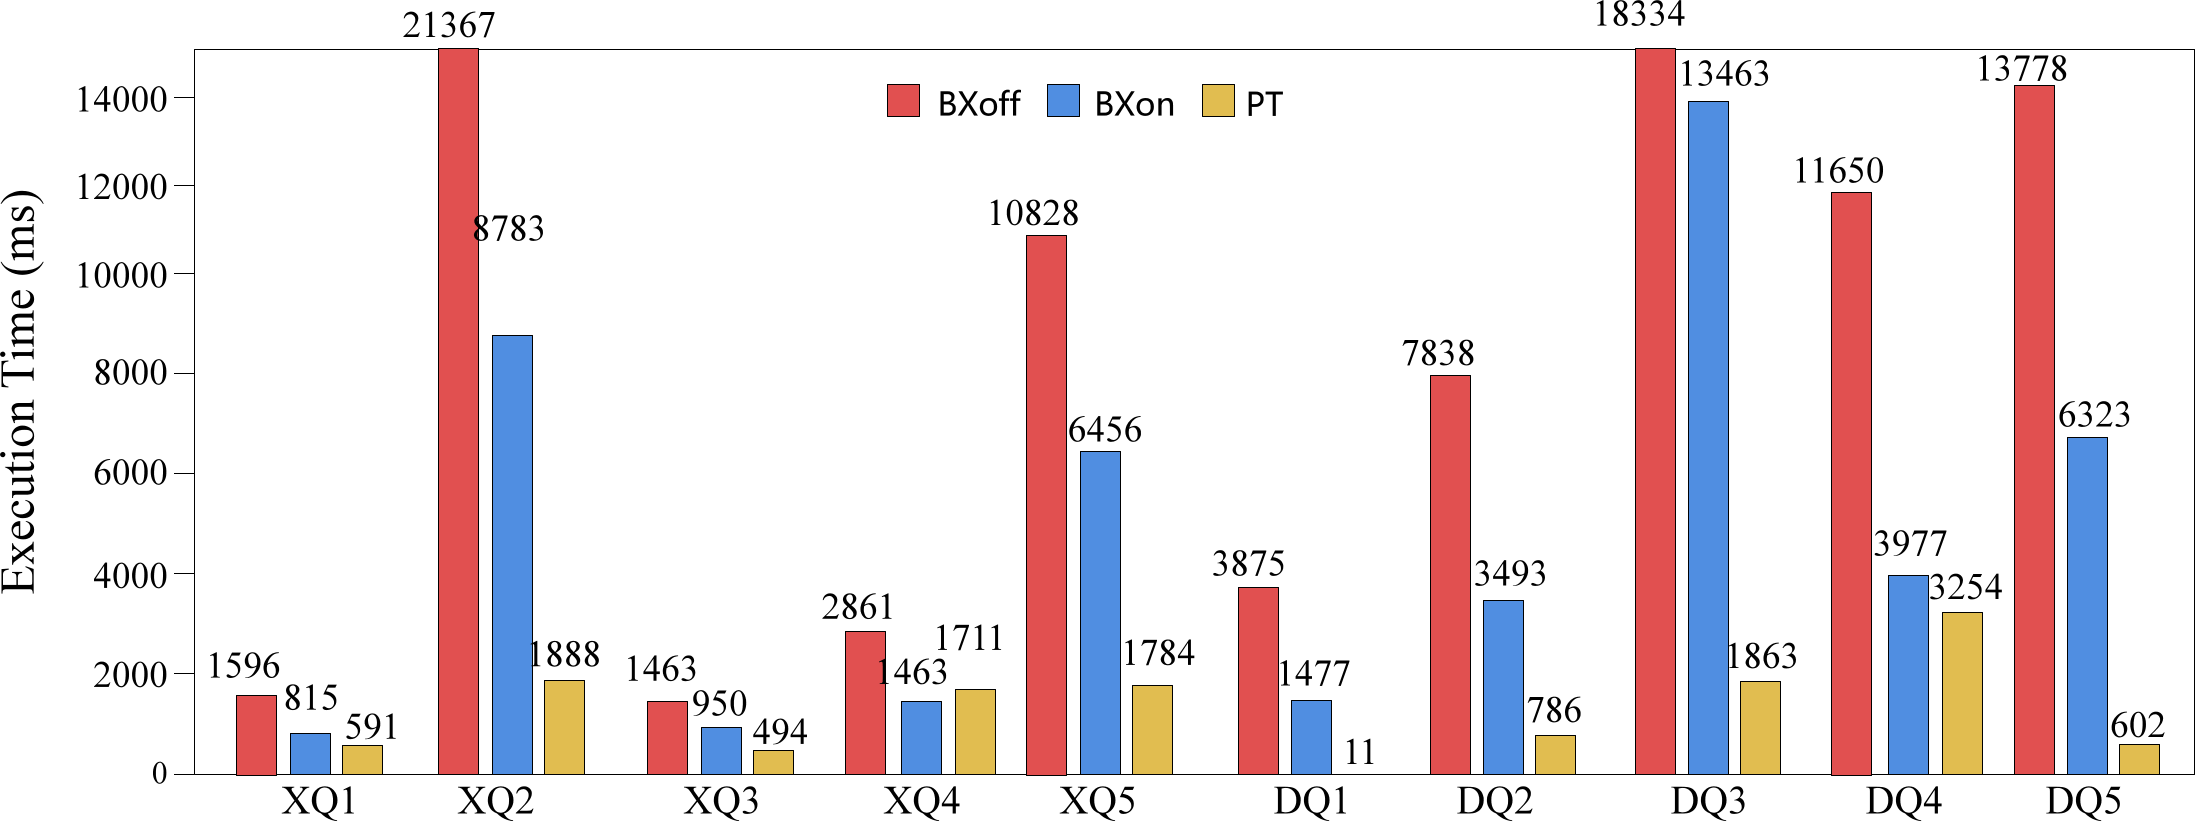
\includegraphics[width=.8\linewidth]{partialtree/figures/query.png}
%	\caption{Execution time of queries on XMark (with factor 100) and DBLP.}
%	\centering
%	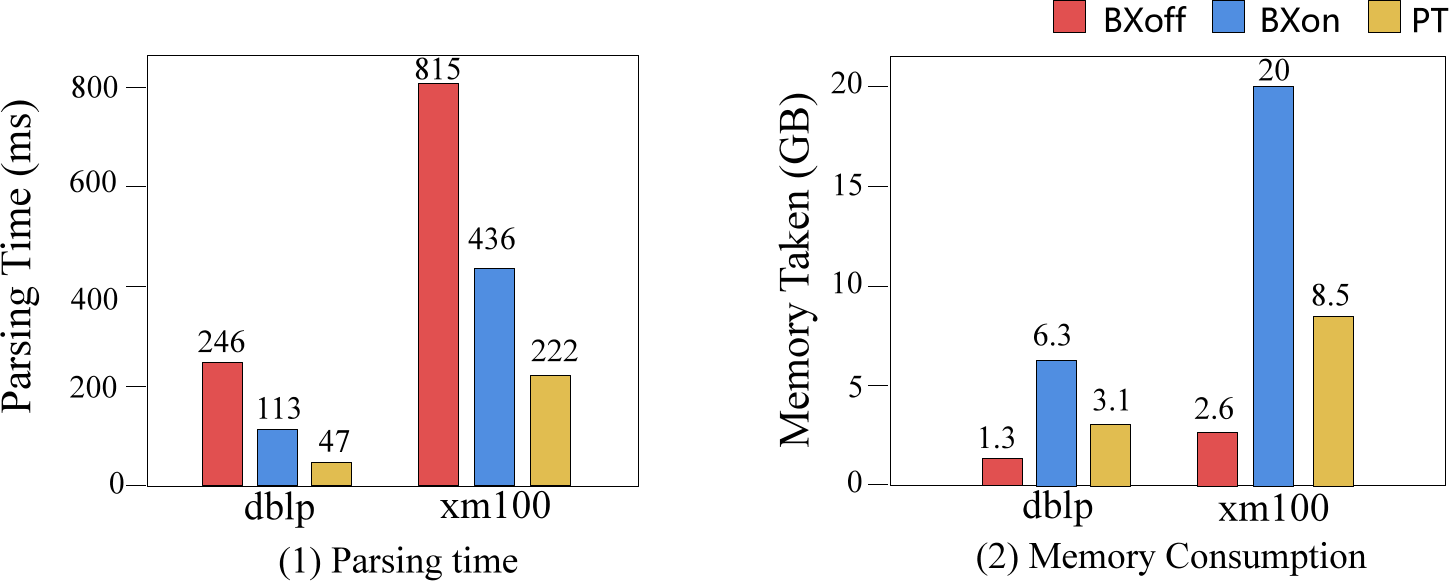
\includegraphics[width=.7\linewidth]{partialtree/figures/parsing.png}
%	\caption{Parsing time and memory taken.}
%	\label{fig:parsing}
%\end{figure}


\begin{table}
	\small
	\caption{Statistics of XML dataset.}
	\label{tab:datasets}
	\begin{tabular}{c|c|c|c|c}
		\hline
		Datasets & dblp.xml & xm100.xml & xm2000.xml & uniprot.xml \\
		\hline \hline
		Nodes & 43,131,420 & 163,156,531 & 3,262,490,248 & 7,891,267,994 \\
		\hline
		Attributes & 10,885,411 & 42,257,706 & 845,072,591 & 9,254,412,578 \\
		\hline
		Values & 39,642,166 & 67,254,767 & 1,344,932,943 & 1,490,598,653 \\
		\hline
		Total & 93,658,997 & 272,669,004 & 5,452,495,782 & 18,636,279,225 \\
		\hline
		\# of tags & 47 & 77 & 77 & 82 \\
		\hline
		Size $($byte$)$ & 1,912,866,012 & 11,758,954,863 & 236,138,315,428 & 383,954,056,809 \\
		\hline
		Depth & 6 & 13 & 13 & 7 \\
		\hline
	\end{tabular}
    \vspace{10px}
	\caption{Queries used in the experiments.}
	\begin{tabular}{c|c|l}
		\hline \hline
		Name & Dataset & Query  \\
		\hline
		XQ1 & xmark & /site/closed\_auctions/closed\_auction[annotation/ \\
		&&description[text/keyword]]\\
		\hline
		XQ2 & xmark & /site//keyword/ancestor::mail \\
		\hline
		XQ3 & xmark & /site/open\_auctions/open\_auction  \\
		&&/bidder[1]/increase\\
		\hline
		XQ4 & xmark & /site/people/person/name/following-sibling::emailaddress \\
		\hline
		XQ5 & xmark & /site/open\_auctions/open\_auction[bidder\\
		&&/following-sibling::bidder]/reserve\\
		\hline
		DQ1 & dblp & /dblp//i/parent::title\\
		\hline
		DQ2 & dblp & //author/ancestor::article \\
		\hline
		DQ3 & dblp & /dblp//author/following-sibling::author \\
		\hline
		DQ4 & dblp & //author[following\textemdash sibling::author] \\
		\hline
		DQ5 & dblp & /dblp/article/title/sub/sup/i/following::author \\
		\hline
		UQ1 & uniprot & /entry[comment/text]/reference[citation \\
		&&/authorList[person]]//person\\
		\hline
		UQ2 & uniprot & /entry//fullName/parent::recommendedName \\
		\hline
		UQ3 & uniprot & /entry//fullName/following::gene \\
		\hline
		UQ4 & uniprot & //begin/ancestor::entry\\
		\hline
		UQ5 & uniprot & //begin/parent::location/parent::feature/parent::entry \\
		\hline
	\end{tabular}
\end{table}


\begin{table}[t]
	\centering
	\caption{Evaluation by one EC2 instance}
	\label{tab:singeval}
	\begin{tabular}{c|c|c|c|c|c|c|c|c|c|c}
		\hline \hline
		Dataset  & \multicolumn{5}{c|}{xmark10.xml} & \multicolumn{5}{c}{dblp.xml} \\ \hline
		Time     & \multicolumn{5}{c|}{8.5}          & \multicolumn{5}{c}{47}       \\ \hline
		Memory   & \multicolumn{5}{c|}{222}          & \multicolumn{5}{c}{3.1}       \\ \hline
		Query    & XQ1  & XQ2   & XQ3 & XQ4  & XQ5  & DQ1 & DQ2 & DQ3  & DQ4  & DQ5 \\ \hline
		Time(ms) & 591  & 1888  & 494 & 1771 & 1784 & 11  & 786 & 1863 & 3254 & 602 \\ \hline
	\end{tabular}
    \vspace{10px}
	\caption{Evaluation by multiple EC2 instance}
	\centering
	\label{tab:multieval}
	\begin{tabular}{c|c|c|c|c|c|c|c|c|c|c}
		\hline \hline
		Dataset	&	\multicolumn{5}{|c|}{xm2000.xml}     & \multicolumn{5}{c}{unirpot.xml}       \\
		\hline
		Loading (ms)	&	\multicolumn{5}{|c|}{210}     & \multicolumn{5}{c}{379}       \\
		\hline
		Memory (GB)	&	\multicolumn{5}{|c|}{173}     & \multicolumn{5}{c}{560}       \\
		\hline
		Query	& QX1      & XQ2     & QX3      & QX4      & QX5      & UX1      & UX2      & UX3      & UX4      & UX5      \\
		\hline
		Time Taken (ms) & 5951 & 819 & 1710 & 1168 & 3349 & 2573 & 2408 & 1324 & 5909 & 6220\\
		\hline
	\end{tabular}
\end{table}



\subsection{Evaluate Queries on a Single EC2 Instance}

This experiment is to investigate the query performance on a single EC2
instance. In this case, we use the whole input XML document as a chunk and only
one partial tree generated from the chunk. Thus the queries are evaluated in
serial. The results show that for both datasets, it can process the queries
in 100s ms to several seconds. These reaults is helpful for us to understand
the query performance of partial tree in serial.


\subsection{Evaluate Queries on Multiple EC2 Instances}

In this experiment, we investigate the query performance processing very large
XML document using multiple EC2 instances. We use UniProtKB and XMark(with
factor 2000) as experimental data. The results are shown in
Table~\ref{tab:multieval}. In the parsing phase, for 0.545 billion and 1.86
billion elements, each of which takes 31 bytes, the memory consumption should
157 GB and 537 GB respectively. The experimental results show the memory
consumption are 173 and 560 GB, which are close to our analysis.  The overheads
is some intermediate data generated during construction. The parsing times as
shown in Table 3 are relatively short with regard to the data sizes. The
evaluating results for XQ1 to XQ5 in Table~3 show that  the query times are just
a few seconds for evaluating 220 GB and 358 GB XML data.  Besides, the loading
times are just 210s and 379s.  The throughput is around 1 GB/s. For comparison,
PP-Transducer~\cite{OgTP13} achieved the best throughput of 2.5 GB/s by using 64
cores. Although it is faster than ours, the queries we can process are more
expressive than PP-transducer, which does not support order-aware queries.
